Bluetooth ist ein Industriestandard für die Übertragung von Daten per Funk, dessen Intention die Reduzierung von Kabelverbindungen an mobilen sowie stationären Geräten war. Wichtige Eigenschaften der Technologie sind vor allem ein niedriger Energieverbrauch und niedrige Herstellungskosten der Hardware. Seit 1998 wird Bluetooth von der Bluetooth Special Interest Group (SIG) entwickelt und ist seit 2002 von der Organisation Institute of Electrical and Electronics Engineers (IEEE) standarisiert \cite{IEEE}.
% QUELLE https://standards.ieee.org/standard/802_15_1-2002.html)

Es agiert im lizenzfreien ISM-Band (Industrial, Scientific and Medical Band) von 2,4 GHz. 
% TODOOPT QUELLE
% BR/EDR: BT Specification 4.0 PDF S. 124, 1.1 Overview of BR/EDR Operation, 1. Absatz
% LE: BT Specifiaction 4.0 PDF S. 126, 1.2 OVERVIEW OF BLUETOOTH LOW ENERGY OPERATION, 1. Absatz
Zur Reichweite kann keine genaue Aussage getroffen werden, da diese von vielen Parametern wie beispielsweise der Sendeleistung und Einflüssen aus der Umwelt abhängt. Um trotzdem einen Eindruck zu gewinnen, kann für bestimmte Bedingungen und Konfigurationen die maximale Reichweite mithilfe eines Tools \cite{BtRangeTool} der SIG ermittelt werden. Dabei variieren die Ergebnisse von ca. einem Meter bis hin zu mehr als 1000 Metern.
% QUELLE https://www.bluetooth.com/learn-about-bluetooth/key-attributes/range/
\\\\
Grundlegend unterscheidet sich Bluetooth seit der Version 4.0 von 2010 in die zwei Systeme Basic Rate (BR) und Low Energy (LE), wobei LE darauf ausgelegt ist weniger Energie als BR zu benötigen. Die neuste Bluetooth-Version ist die Version 5.2, die wie jede Version abwärtskompatibel ist. Jedoch sind beide Systeme (BR und LE) bezüglich der Kommunikation miteinander inkompatibel. D.h. implementiert ein Gerät nur das BR-System, kann es keine Daten mit einem Gerät austauschen, das nur das LE-System unterstützt. Demnach ist für LE die Abwärtskompatibilität nur bis zur Version 4.0 gegeben. Desweiteren ist es möglich, dass ein Gerät über beide Systeme verfügt und so die meisten Nutzungsfälle abdeckt. Das BR-System kann mit den Erweiterungen Enhanced Data Rate (EDR) und Alternate Media Access Control and Physical Layer (AMP) genutzt werden, um eine höhere Datenrate zu erreichen. Die einzelnen Systeme und Erweiterungen können entsprechend ihrer Bluetooth-Version die in Tablle \ref{tab: maximale Bitraten BT} dargestellten Datenraten erreichen.\\

\begin{table}
    \begin{tabular}[h]{|l|l|l|}
    \hline
    \textbf{System/Erweiterung} & \textbf{max. Bitrate (Version 4.0)} & \textbf{max. Bitrate (Version 5.2)} \\
    \hline
    BR          & 1 Mb/s \cite{BtSpec4.0_124}               & 1 Mb/s \cite{BtSpec5.2_188}           \\
    \hline
    BR/EDR      & 2 Mb/s bis 3 Mb/s \cite{BtSpec4.0_124}    & 2 Mb/s bis 3Mb/s \cite{BtSpec5.2_188} \\
    \hline
    802.11 AMP  & 24 Mb/s \cite{BtSpec4.0_123}              & 52 Mb/s \cite{BtSpec5.2_187}          \\
    \hline
    LE          & 1 Mb/s \cite{BtSpec4.0_126}               & 2 Mb/s \cite{BtSpec5.2_190}           \\
    \hline
    % QUELLE
    % BT Specification 4.0 PDF S. 124, 1.1 Overview of BR/EDR Operation, 1. Absatz
    %                          S. 126, 1.2 OVERVIEW OF BLUETOOTH LOW ENERGY OPERATION, 1. Absatz
    % BT Specification 5.2 PDF S. 188 1.1 Overview of BR/EDR Operation, 1. Absatz
    %                          S. 190, 1.2 OVERVIEW OF BLUETOOTH LOW ENERGY OPERATION, 1. Absatz
    \end{tabular}
    \caption[Maximale Bitraten der Bluetooth-Systeme]{Maximale Bitraten der Bluetooth-Systeme}
    \label{tab: maximale Bitraten BT}
\end{table}

\textit{Da Bluetooth Low Energy (BLE) ein zentraler Bestandteil dieser Arbeit ist, bezieht sich der Autor von nun an nur auf dieses und nicht mehr auf Bluetooth im Allgemeinen. D.h., dass Bluetooth Classic, welches BR/EDR und AMP beschreibt, nur noch behandelt wird, wenn das BR-System oder eine seiner Erweiterungen explizit erwähnt werden.}
\\\\
Die Architektur eines Bluetooth-Systems unterteilt sich in einen Host und in einen oder mehrere Controller. Ein Host ist eine logische Entität, definiert als alle Schichten unterhalb der nicht zu Bluetooth gehörigen Profile (Protokolle) und oberhalb des Host-Controller-Interface (HCI). Ein Controller ist eine logische Entität, definiert als alle Schichten bzw. Funktionsblöcke unterhalb des HCI. Der Aufbau setzt sich immer aus genau einem primären Controller und optional aus sekundären Controllern zusammen. Dabei kann die Rolle des primären Controllers entweder durch einen BR/EDR-Controller, einen LE-Controller oder durch eine Kombination aus BR/EDR- und LE-Controller eingenommen werden, während die Rolle eines sekundären Controllers nur durch einen AMP-Controller besetzt werden kann. In Abb. \ref{fig: kombinationen aus host und controller} sind einige Varianten skizziert. 
% TODOOPT QUELLE BT Specification 4.0, PDF S.123 f.

\begin{figure}
    \centering
    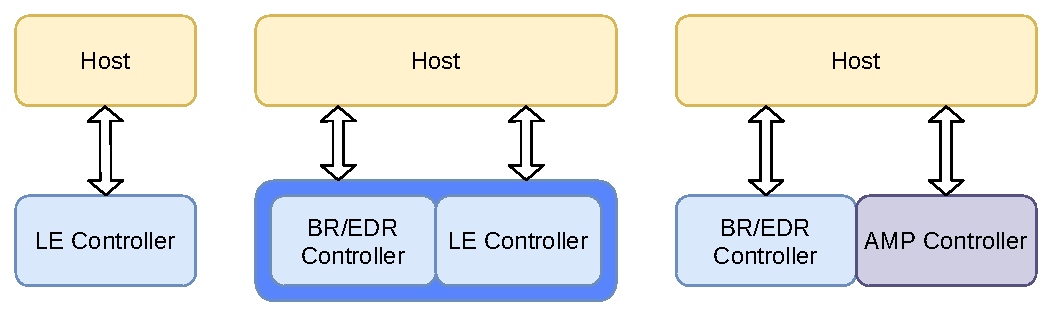
\includegraphics[width=0.9\linewidth]{graphics/kombination_host_controller.pdf}
    \caption{Kombinationen aus Host und Controller \cite{BtSpec4.0_fig_124}}
    \label{fig: kombinationen aus host und controller}
\end{figure}
% QUELLE BILD BT Sepcification 4.0, PDF S. 124

Zur Veranschaulichung der Architektur bezüglich eines LE-Systems ist in der Abb. \ref{fig: host controller architektur} die Zusammensetzung aus Host und Controller mit deren Schichten bzw. Protokollen festgehalten, die in den folgenden Sektionen \ref{sec: le controller} und \ref{sec: le host} thematisiert werden. Über dem Host befindet sich die Anwendungsschicht.

\begin{figure}
    \centering
    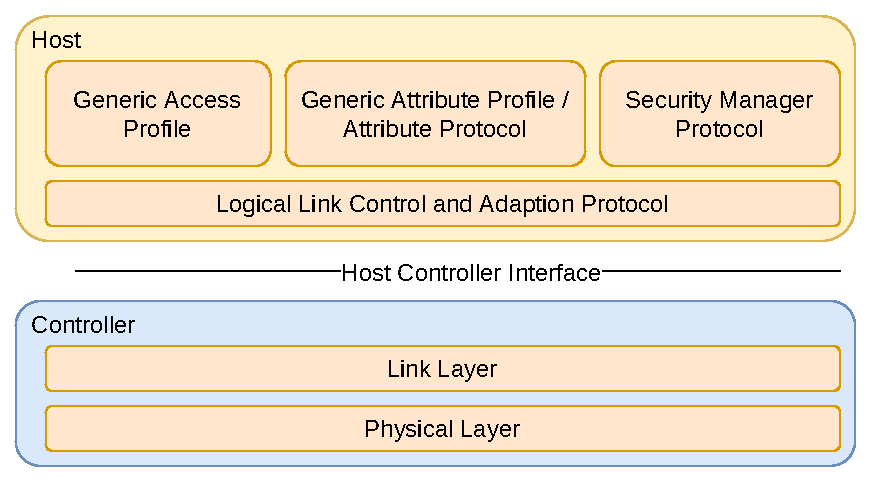
\includegraphics[width=0.7\textwidth]{graphics/host_controller_hci.pdf}
    \caption[Bluetooth Low Energy Architektur von Host und Controller]{Bluetooth Low Energy Architektur von Host und Controller \cite{BtSpec4.0_fig_137}}
    \label{fig: host controller architektur}
\end{figure}